\section{Experimental evaluation}

% \mpaga{Manca una sezione nella quale presentiamo i principali obiettivi degli esperimenti}
Our experiments are designed to answer four questions. (\textbf{RQ1}) \emph{Scaling}: how does performance evolve as the number of tables grows, in both parallel and sequential settings? (\textbf{RQ2}) \emph{Numerical heterogeneity}: to what extent do unit discrepancies and quantitative computation degrade accuracy, and is this effect domain-dependent? (\textbf{RQ3}) \emph{Utility}: beyond evaluation, can \name{}-generated data serve as effective training supervision? (\textbf{RQ4}) \emph{Question correctness}: what is \name{}'s percentage of correctly generated questions?
We address these through controlled benchmarks in the financial and environmental domains, and validate our findings on perturbed real tables in \S\ref{app:generating_non_rel}.

\subsection{Baselines}

We evaluate four LLMs with different scales and access settings, by providing them the NL question and the generated non-relational views:
\texttt{gpt-5-mini}, \texttt{Qwen3.5-122B-A10B-FP8} (Qwen 122B),
\texttt{Qwen3.5-35B-A3B-FP8} (Qwen 35B), and \texttt{Qwen3.5-9B} (Qwen 9B).
This covers one strong closed model and open-weight models of different sizes, testing whether failures exposed by \name are model-family specific or persist across scale.
All models use zero-shot Chain-of-Thought~\cite{cot}, with \emph{thinking} enabled, temperature equal to 0 and a token budget of 16384 for Qwen; details are in \S\ref{sec:appendix}. Additional experiments with Program-of-Thoughts prompting~\cite{pot} are detailed in \S\ref{sec:exp_train}.

\subsection{Metrics}
\label{sec:metrics}

We report accuracy using normalized exact match (EM) at 2-decimal precision against the automatically computed gold answer, after removing superficial formatting differences, such as surrounding whitespace and thousands separators. Accuracy is the percentage of examples whose normalized prediction matches the gold answer.

\subsection{Datasets}

We generate \name\ instances in two domains, environmental and finance, using \texttt{gpt-5-mini} as its internal LLM. Unless otherwise stated, evaluation covers parallel and sequential questions over 2, 3, and 5 tables, with parallel questions also scaled to 10 and 20 tables. We request 50 instances for each combination of domain, table count, aggregation operator (sum, average, superlative), and, for parallel questions, same- or mixed-unit setting. Perturbations are applied randomly but compositionally: each larger benchmark extends the next smaller one, so 3-table instances reuse 2-table inputs, and so on. Thus, every ablation reuses the same inputs, varying only the studied property. In all experiments, rendered views are capped at $10 \times 10$ cells to control for table-size variance. The cap is a generation parameter, and larger views can be rendered by relaxing it. 
%In all experiments, rendered views are capped at $10 \times 10$ cells to keep inputs compact. 
After discarding generations that fail the schema-format check (\S\ref{subsec:data-generation}, \S\ref{sec:semantic_constraints}), we obtain 2{,}322 parallel and 840 sequential instances; further statistics are in \S\ref{sec:data_statistics}.
% \mlc{non so se vadano contestualizzate meglio le failure cases di \name: io pensavo di metterle in appendice} \mpaga{Inserirei una tabella con statistiche sulle domande generate distinguendo num tabelle, parallel/sequential, e se necessario altre dimensioni (es., comparative vs quantitative)...un po' come fatto in GRI-QA} \mlc{io metterei una tabella in appendice che riassume le statistiche di tutti i dati usati, anche quelli di finetuning. Tabella: \autoref{tab:data_statistics}}

%Each configuration contains [N] instances per domain, balanced across the aggregation operators (sum, average, superlative) and, for parallel questions, across same-unit and mixed-unit settings. [comment: state total number of generated instances, e.g. "yielding X instances in total"]

\subsection{Discussion}
\label{sec:discussion}

% \stitle{(\textbf{RQ1}) Scaling collapses performance.}
% % \mpaga{As a first experiment, we study how scaling the number of tables affects LLM performance in both parallel and sequential multi-table settings. The results are reported in~\autoref{fig:scaling_parallel_sequential}. In both reasoning regimes, accuracy degrades sharply as the number of tables increases.}
% As shown in~\autoref{fig:scaling_parallel_sequential}, accuracy decreases as the number of tables increases in both parallel and sequential settings.
% % For parallel questions, moving from 2 to 20 tables reduces performance by 39.6 points for \texttt{gpt-5-mini}, and by 26.1, 32.8, and 38.3 points for Qwen 122B, Qwen 35B, and Qwen 9B, respectively (\autoref{fig:parallel_scaling}). The largest degradation appears in the 10- and 20-table settings: \texttt{gpt-5-mini} is strongest with few tables, reaching 95.53 accuracy points at 3 tables, but drops to 52.61\% at 20 tables. At the same point, Qwen 122B, Qwen 35B, and Qwen 9B obtain 64.90, 56.42, and 26.74 points, respectively.
% In parallel scenarios, scaling from 2 to 20 tables causes substantial drops across all models (\autoref{fig:parallel_scaling}): \texttt{gpt-5-mini} decreases by 39.6 points, while Qwen 122B, Qwen 35B, and Qwen 9B lose 26.1, 32.8, and 38.3 points, respectively. Although \texttt{gpt-5-mini} achieves the highest performance with few tables (95.53\% at 3 tables), accuracy collapses at larger scales, reaching only 52.61\% at 20 tables. At the same point, Qwen 122B, Qwen 35B, and Qwen 9B obtain 64.90\%, 56.42\%, and 26.74\%, respectively.


% % Sequential questions show the same trend.
% % Increasing the lookup chain from 2 to 5 tables reduces accuracy by 32.5 points for \texttt{gpt-5-mini}, and by 28.8, 24.6, and 10.9 points for Qwen 122B, Qwen 35B, and Qwen 9B (\autoref{fig:sequential_scaling}).
% % At 5 tables, \texttt{gpt-5-mini} remains the strongest model with 48.37 accuracy points, followed by Qwen 35B and Qwen 122B with 42.97 and 38.21, while Qwen 9B reaches 24.93 points.
% % Overall, \texttt{gpt-5-mini} achieves the best absolute performance, Qwen 122B and Qwen 35B behave similarly, and Qwen 9B is consistently weaker.
% Sequential settings show the same pattern (\autoref{fig:sequential_scaling}): extending the lookup chain from 2 to 5 tables reduces accuracy by 32.5 points for \texttt{gpt-5-mini}, 28.8 for Qwen 122B, 24.6 for Qwen 35B, and 10.9 for Qwen 9B. At 5 tables, performance ranges from 48.37\% for \texttt{gpt-5-mini} to 24.93\% for Qwen 9B.

% % At matched table counts, sequential questions are consistently harder than parallel ones (\autoref{fig:scaling_parallel_sequential}).
% Comparing the two regimes (\autoref{fig:parallel_sequential_penalty}), sequential reasoning is consistently harder than parallel aggregation at matched table counts.
% The average gap grows from 21.6 points with 2 tables to 40.1 points with 5 tables, showing that propagating lookup keys across tables adds difficulty beyond aggregating independent evidence.
% However, the two regimes stress models differently: sequential questions are harder at the same table count, while parallel questions can scale to many more tables, where the scaling collapse makes their difficulty comparable to shorter sequential chains.

\begin{figure}[t]
    \centering
    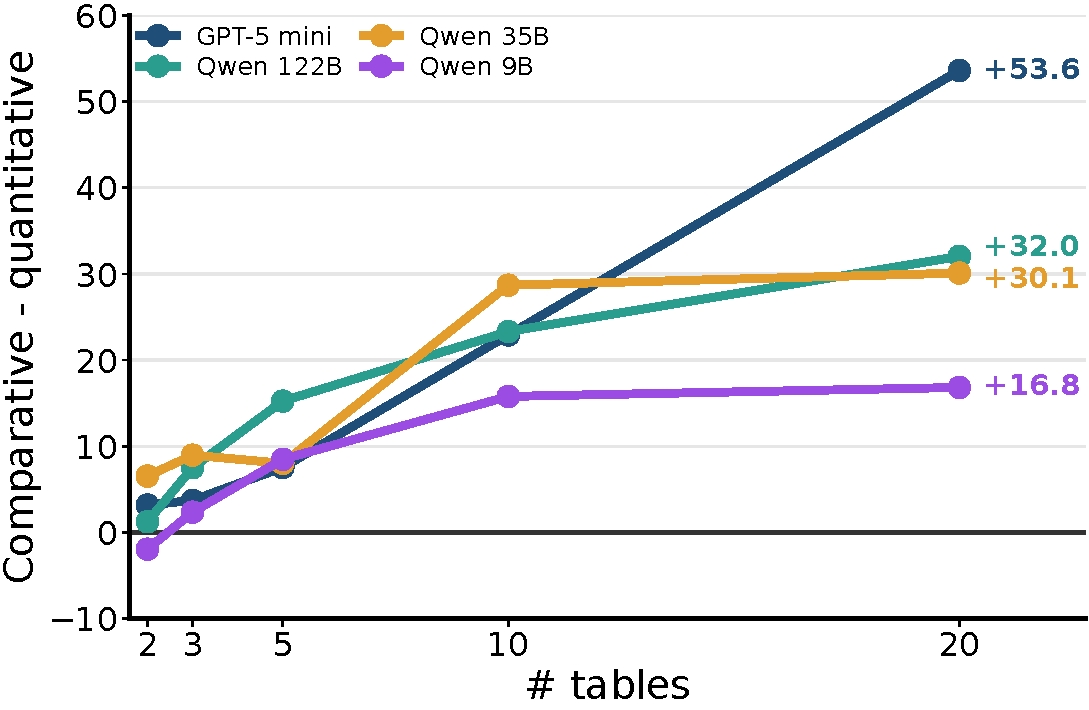
\includegraphics[width=\linewidth]{img/quant_vs_rel.pdf}
\caption{Performance gap between comparative and quantitative parallel questions as table count increases, averaged over domains and unit settings.
%Quantitative questions are harder, especially when many table-specific numerical values are extracted and aggregated.
}

    % \caption{
    % Performance gap between relational and quantitative parallel questions as the number of tables increases.
    % Quantitative questions are harder than relational ones, especially when many table-specific numerical values must be extracted and aggregated. %\mpaga{cavolata: perché sfondo grigio, quando le altre sono bianche?}
    % }
    \label{fig:question_type_gap}
\end{figure}

\stitle{(\textbf{RQ1}) Scaling collapses performance.}
As shown in \autoref{fig:scaling_parallel_sequential}, \emph{accuracy degrades sharply as the number of tables grows}, in both parallel and sequential regimes. For parallel questions, scaling from 2 to 20 tables costs \texttt{gpt-5-mini} 39.6 points, and Qwen 122B, 35B, and 9B 26.1, 32.8, and 38.3 points (\autoref{fig:parallel_scaling}). \texttt{gpt-5-mini} leads with few tables (95.53\% at 3) but collapses to 52.61\% at 20, where Qwen 122B, 35B, and 9B reach 64.90\%, 56.42\%, and 26.74\%. Sequential accuracy follows the same trend: extending the chain from 2 to 5 tables costs 32.5 points for \texttt{gpt-5-mini} and 28.8, 24.6, and 10.9 points for Qwen 122B, 35B, and 9B (\autoref{fig:sequential_scaling}). 
Additionally, \emph{sequential reasoning is harder than parallel aggregation.} Because it forces the model to propagate lookup keys across tables rather than combine independent evidence, sequential accuracy drops even faster per table, with the gap over parallel questions widening from 21.6 points at 2 tables to 40.1 at 5 (\autoref{fig:parallel_sequential_penalty}). The two regimes thus stress models differently: sequential chains are harder per table, whereas parallel questions scale to far more tables, where the collapse makes them comparably difficult.


% \stitle{Quantitative questions create a bottleneck.}
% \stitle{(\textbf{RQ2}) Quantitative reasoning and unit heterogeneity are a major bottleneck.}
% The observed scaling collapse is largely driven by quantitative questions.
% In \autoref{fig:question_type_gap}, we report the average gap between relational and quantitative parallel questions.
% All models exhibit a consistent trend: the gap increases as the number of tables grows, indicating that numerical computation becomes progressively harder when more table-specific values must be extracted and aggregated.
% At 20 tables, \texttt{gpt-5-mini} reaches the largest degradation, with quantitative questions underperforming relational ones by 53.6 points.
% The same pattern holds for Qwen 122B, Qwen 35B, and Qwen 9B, with gaps of 32.0, 30.1, and 16.8 points, respectively.
% % Overall, as scaling collapse becomes more severe, questions requiring precise numerical computation account for a larger share of the errors.
% Overall, quantitative reasoning accounts for an increasing share of errors as table complexity grows.



% % \stitle{Unit heterogeneity leads to domain-specific degradation.}
% This effect is further amplified by unit heterogeneity. As shown in \autoref{fig:unit_heterogeneity}, adding heterogeneous units on top of the same parallel settings leads to additional performance drops, with a strong domain dependence.
% % Adding heterogeneous units of measurement on top of the perturbations used in \autoref{fig:parallel_scaling} further reduces performance on parallel questions.
% % \autoref{fig:unit_heterogeneity} reports the average drop across table counts, split by domain.
% The effect is particularly pronounced in the environmental domain, where performance decreases by 50.1 points for \texttt{gpt-5-mini}, and by 45.3, 46.8, and 38.9 points for Qwen 122B, Qwen 35B, and Qwen 9B, respectively.
% % : performance decreases by 50.1 points for \texttt{gpt-5-mini}, and by 45.3, 46.8, and 38.9 points for Qwen 122B, Qwen 35B, and Qwen 9B, respectively.
% In contrast, the same perturbation is considerably less severe in finance, with drops of 6.7, 7.3, 9.9, and 14.2 points.
% This suggests that unit heterogeneity is not mere formatting, but a domain-dependent reasoning challenge.
% % Environmental quantities may require conversions across heterogeneous physical units, such as gallons to liters in water-consumption questions, while the considered financial setting mostly involves decimal-scale conversions, such as thousands or billions.
% Environmental questions often involve heterogeneous physical conversions (e.g., gallons to liters), whereas finance mostly uses scale conversions (e.g., thousands to billions).
% Thus, robustness to numerical representations may not transfer across domains: domain-specific table conventions can induce distinct failure modes that affect model performance~\cite{clariesg}.

\begin{figure}[t]
    \centering
    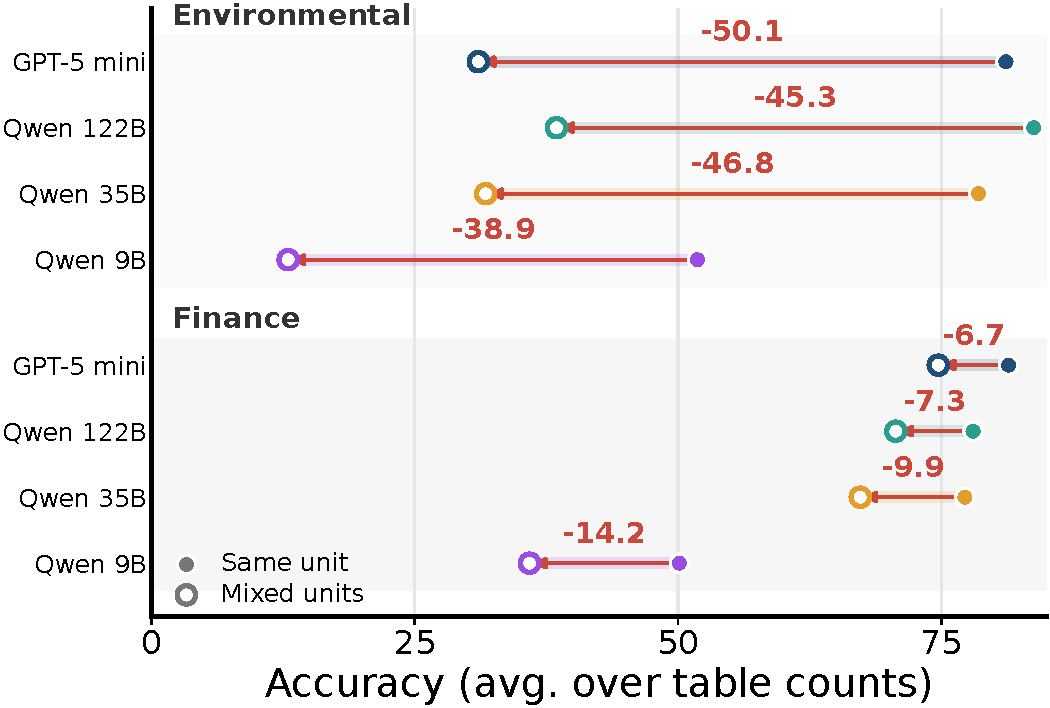
\includegraphics[width=\linewidth]{img/unit_heterogeneity.pdf}

    \caption{
    Per-model, per-domain accuracy drop from unit heterogeneity on parallel questions.
    %Effect of unit heterogeneity on parallel questions, showing the per-model, per-domain accuracy drop.
    %Effect of unit heterogeneity on parallel questions. Red arrows indicate the drop for each model and domain, averaged across different table counts.
    }
    \label{fig:unit_heterogeneity}
\end{figure}

\stitle{(\textbf{RQ2}) Quantitative reasoning and unit heterogeneity are a major bottleneck.}
The scaling collapse is largely driven by precise numerical computation, as \emph{quantitative reasoning drives the collapse.} The gap between the accuracy over comparative and quantitative parallel questions widens with table count for every model (\autoref{fig:question_type_gap}): at 20 tables it peaks at 53.6 points for \texttt{gpt-5-mini}, and reaches 32.0, 30.1, and 16.8 points for Qwen 122B, 35B, and 9B, so quantitative questions account for a growing share of errors. This effect is amplified by unit heterogeneity, which causes \emph{a domain-dependent collapse.} As shown in \autoref{fig:unit_heterogeneity}, in the environmental domain, where questions often require physical conversions (e.g., gallons to liters), it costs \texttt{gpt-5-mini} 50.1 points and Qwen 122B, 35B, and 9B 45.3, 46.8, and 38.9, whereas in finance, dominated by scale conversions (e.g., thousands to billions), the same perturbation is far milder (6.7, 7.3, 9.9, and 14.2 points). %As a result, domain-specific conventions induce distinct failure modes towards robustness to numerical representation~\cite{clariesg}.
Robustness to numerical representation is thus domain-specific, as each unit convention induce distinct failure modes~\cite{clariesg}.
%Robustness to numerical representation therefore does not transfer across domains, as domain-specific conventions induce distinct failure modes~\cite{clariesg}.


% \stitle{Perturbed parallel and sequential questions are difficult to synthesize from real tables.}
% Not all perturbations and numerical question types can be obtained by transforming real relational tables.
% To test this, we extracted databases from Spider, BIRD, and BEAVER, obtaining 2,096 relational tables, and retained only the 148 tables with at least one floating-point attribute. \mpaga{Non capisco quali proprietà stiamo cercando nelle tabelle? Sembra che cerchiamo tabelle con almeno un attributo float e mi sembra impossibile che rimangano solo 148 tabelle o è veramente così? Filtro su num minimo colonne (3) e righe (9)}
% For each table, we attempted to construct a pivoted view by selecting the attributes that maximize density, defined as the fraction of non-\texttt{NaN} cells in the resulting pivot.
% We do not search over subsets of attribute values, since this would make the pivot search combinatorial and impractical for tables with many tuples.

% As shown in \autoref{fig:real_table_feasibility}, even a simple one-level row and column pivot discards 95.3\% of the candidates, while requiring at least two hierarchical levels on either rows or columns discards 98.6\%.
% Thus, common non-relational perturbations such as dense pivots and hierarchical headers are rarely directly applicable to real relational sources.
% The constraint becomes even stronger for parallel and sequential multi-table scenarios, which require compatible evidence values, valid lookup chains, sufficient table sizes, and, when units are perturbed, convertible numerical quantities.
% By generating the latent source and the perturbed views jointly, \name satisfies these constraints by construction.

% \stitle{Non-relationalization amplifies errors in multi-table settings, even in real tables.} Starting from the two relational tables that support at least two hierarchical levels on rows or columns, we extend the source pool with five additional tables from three Kaggle databases.
% We then use \name to apply all structural and cell-level perturbations, and generate both single-table instances and 3-table parallel scenarios.
% This yields 108 single-table and 84 multi-table instances, repeated over three seeds for more stable estimates.

% \autoref{fig:rel_to_nonrel} shows that non-relationalization consistently reduces accuracy, but the drop is much larger in the multi-table setting.
% In single-table instances, performance decreases by 5.7 points for \texttt{gpt-5-mini}, and by 5.5, 7.6, and 13.1 points for Qwen 122B, Qwen 35B, and Qwen 9B.
% In multi-table instances, the drops increase to 19.8, 25.4, 28.2, and 46.8 points.
% Importantly, this cannot be explained by the number of tables alone: in the clean relational setting, performance does not decrease when moving from single-table to multi-table inputs.
% The degradation therefore comes from the interaction between multi-table reasoning and non-relational variability across views.

% \begin{table}[t]
% \centering
% \small
% \setlength{\tabcolsep}{2.5pt}
% \begin{tabular}{@{}l cc cc cc c@{}}
% \toprule
% \multirow{2}{*}{Train data} & \multicolumn{2}{c}{2} & \multicolumn{2}{c}{3} & \multicolumn{2}{c}{5} & \\
% \cmidrule(lr){2-3}\cmidrule(lr){4-5}\cmidrule(lr){6-7}
% & rel & qnt & rel & qnt & rel & qnt & avg \\
% \midrule
% None & 18.3 & 9.3 & 17.1 & 9.7 & 9.2 & 0.0 & 10.6 \\
% \midrule
% \name (fin) & 22.3 & 46.4 & 23.3 & 17.7 & 14.7 & 5.8 & 21.7$^{+11.1}$ \\
% \name (env) & 35.5 & 50.0 & 35.3 & 18.3 & 25.8 & 5.0 & 28.3$^{+17.3}$ \\
% \midrule
% TAT-QA & 33.1 & 46.4 & 28.3 & 19.0 & 13.3 & 4.2 & 24.1$^{+13.1}$ \\
% GRI-QA & 73.5 & 44.9 & 53.0 & 15.0 & 32.5 & 3.3 & 37.0$^{+25.2}$ \\
% \name (env) + GRI-QA & 83.5 & 52.9 & 70.0 & 15.0 & 48.1 & 12.5 & 47.0$^{0.00}$ \\
% \bottomrule
% \end{tabular}
% \caption{Accuracy of Qwen2.5-14B-Instruct fine-tuned, evaluated on the GRI-QA test split, by number of input tables (2/3/5) and question type (relational, quantitative), averaged over 3 seeds. Superscripts report the average gain over the non-finetuned baseline (None).}
% \label{tab:finetuning}
% \end{table}

% \stitle{(\textbf{RQ3}) Data generated by \name\ has functional utility.} 
% To evaluate the utility, 
% % of \name-generated data for training, 
% we fine-tune \texttt{Qwen2.5-14B-Instruct} using correct \texttt{gpt-5-mini} reasoning traces derived from \name instances. %\mpaga{Concretely, we first generate parallel multi-table questions with \name in configurations with 2, 3, and 5 tables, across both financial and environmental domains and under both matched and mixed unit settings. We then evaluate \texttt{gpt-5-mini} on these instances and retain only those for which it produces the correct final answer. For each selected instance, we extract the corresponding reasoning trace, yielding a dataset of 440 training records.}
% % We finetune a no-thinking Qwen2.5-14B-Instruct on \texttt{gpt-5-mini} generated reasoning traces to test whether \name-generated data is also useful for training. As a test benchmark we use GRI-QA~\cite{1.16}, which poses relational and quantitative questions over 2, 3, and 5 environmental tables. 
% As an evaluation benchmark, we use GRI-QA~\cite{1.16}, which consists of relational and quantitative questions over 2-, 3-, and 5-table environmental settings.
% We compare several training regimes: no finetuning, \name-generated 2-, 3- and 5-table training data, and real data (financial single-table TAT-QA~\citealp{1.9} and the GRI-QA train split). %\mpaga{, with real-world datasets subsampled and matched in size to the \name-generated training set.}. 
% For all finetuning settings, we restrict the training data to 440 randomly sampled instances.
% %\mlc{non so se abbia senso spiegare il motivo dei 440: è il numero di istanze di training corrette del setting di \name environmental (il mixed units ha pochi reasoning trace corretti). Stessa cosa per GRI-QA: i sample multi-table corretti non sono tantissimi, e più aumento, più diminuisce il test set utilizzabile per l'esperimento.}.
% Results are reported in \autoref{tab:finetuning}. 
% All regimes outperform the non-finetuned baseline (+11.1 to +25.2 on average), with gains strongly depending on domain alignment: environmental data consistently outperforms financial data due to better match with the GRI-QA test domain.
% % All regimes improve over the no-finetuning baseline (+11.1 to +25.2 on average), but the gain is domain-dependent: training on environmental data, matching the GRI-QA test domain, outperforms financial data.
% Notably, \name exposes models to multi-table and quantitative settings largely absent in real single-table benchmarks: while TAT-QA fine-tuning is competitive at 2 tables (43.6 on average over relational and quantitative questions), it degrades sharply with scale (6.3 at 5 tables). In contrast, \name (environmental) shows a more stable trend (15.4 at 5 tables).

% % Crucially, \name\ data covers cases that single-table real benchmarks miss: the TAT-QA–finetuned model is competitive at 2 tables (43.6 average) but collapses as tables increase (6.3 average at 5), whereas \name\ (env) degrades far more gracefully (15.4 average). 
% Finally, the GRI-QA train split, being in-domain, yields the strongest results, yet its gains concentrate on relational rather than quantitative questions, likely reflecting the scarcity of quantitative examples in its training split. This underscores that the scalable, quantitative-rich generation of \name\ is needed to improve numerical reasoning at scale.

\begin{table}[t]
\centering
\small
\setlength{\tabcolsep}{2.23pt}
\begin{tabular}{@{}l cc cc cc c@{}}
\toprule
\multirow{2}{*}{\textbf{Train data}} & \multicolumn{2}{c}{2} & \multicolumn{2}{c}{3} & \multicolumn{2}{c}{5} & \\
\cmidrule(lr){2-3}\cmidrule(lr){4-5}\cmidrule(lr){6-7}
& com & qnt & com & qnt & com & qnt & \textbf{Mean} \\
\midrule
None & 18.3 & 9.3 & 17.1 & 9.7 & 9.2 & 0.0 & 10.6 \\
\midrule
\name (fin) & 22.3 & 46.4 & 23.3 & 17.7 & 14.7 & 5.8 & 21.7$^{+11.1}$ \\
\name (env) & 35.5 & 50.0 & 35.3 & 18.3 & 25.8 & 5.0 & 28.3$^{+17.7}$ \\
\midrule
TAT-QA & 33.1 & 46.4 & 28.3 & 19.0 & 13.3 & 4.2 & 24.1$^{+13.5}$ \\
GRI-QA & 73.5 & 44.9 & 53.0 & 15.0 & 32.5 & 3.3 & 37.0$^{+26.4}$ \\
\midrule
\makecell[l]{\name (env)\\[-1pt]+ GRI-QA} & 83.5 & 52.9 & 70.0 & 15.0 & 48.1 & 12.5 & 47.0$^{+36.4}$ \\
\bottomrule
\end{tabular}
\caption{Accuracy of Qwen2.5-14B-Instruct fine-tuned on different training splits, evaluated on GRI-QA by number of tables and question type (comparative, quantitative), averaged over 3 seeds. Superscripts report the gain over the non-finetuned baseline; std. dev. in \S\ref{app:variance}.
%Accuracy of Qwen2.5-14B-Instruct fine-tuned on different training splits, evaluated on the GRI-QA test split, by number of input tables (2/3/5) and question type (comparative, quantitative), averaged over 3 seeds. Superscripts report the average gain over the non-finetuned baseline. Std. dev. is reported in \S\ref{app:variance}.
}
\label{tab:finetuning}
\end{table}

\stitle{(\textbf{RQ3}) \name-generated data has functional utility.}
% Beyond evaluation, we test whether \name data is useful as training supervision by fine-tuning \texttt{Qwen2.5-14B-Instruct} on \texttt{gpt-5-mini} reasoning traces whose final answer matches the SQL-derived gold answer.
Beyond evaluation, we test whether \name-generated data is useful as training supervision by augmenting it with \texttt{gpt-5-mini} reasoning traces whose final answers match the SQL-derived gold answers, and fine-tuning \texttt{Qwen2.5-14B-Instruct}. 
We evaluate on GRI-QA~\cite{1.16}, which poses parallel comparative and quantitative questions over 2-, 3-, and 5-table environmental settings (\autoref{tab:finetuning}).
Since no comparable multi-table non-relational training set exists, which is the very gap \name targets, we compare against the three most relevant options: the in-domain GRI-QA train split, an out-of-domain single-table set (financial TAT-QA~\citealp{1.9}), and no fine-tuning. The TAT-QA baseline probes a common deployment scenario: a practitioner who needs a multi-table system in a target domain, but lacks in-domain multi-table data, falls back on an available single-table set from another domain. To keep the comparison fair given GRI-QA's limited size, every regime is capped at 440 instances, a cap that is itself a symptom of the data scarcity \name addresses.
All regimes improve over the non-finetuned baseline (+11.1 to +36.4 on average), and two takeaways emerge. First, \emph{in-domain multi-table supervision matters most.} Because both the domain and the reasoning structure of the training data align with the test setting, \name (env) leads out-of-domain TAT-QA at every table count, with the gap widening from +3.0 at 2 tables to +6.7 at 5. TAT-QA collapses as tables accumulate (8.8 average at 5 tables), while \name (env) degrades more gracefully (15.4). Second, \emph{\name complements scarce in-domain data.} As expected, GRI-QA leads \name (env) overall, since it is trained on the same distribution as the test set; however, GRI-QA's train split is skewed toward comparative questions ($\sim$3$\times$ more comparative than quantitative), so the GRI-QA-tuned model stays weak on quantitative reasoning compared to \name (env). Moreover, \name can cheaply supply the multi-table examples GRI-QA's split lacks: combining GRI-QA + \name (env) yields the best model overall (+36.4) and improves performance at \emph{every} table count and question type over GRI-QA alone. This confirms that \name augments rather than merely substitutes for real data, providing the scalable, multi-table supervision that existing benchmarks lack.

% \stitle{(\textbf{RQ4}) Question generation is reliable.} Question generation is the only \name stage that can introduce errors. To estimate its reliability, we manually inspected 10 instances per aggregation operator (sum, average, superlative) in the environmental domain, covering parallel (20 tables, unit-converted) and sequential (5 tables) regimes, for 60 total. As shown in \autoref{tab:correctness}, all parallel instances are correct, while sequential ones average 86.7\%. 
% %The gap reflects a verbalization asymmetry. Parallel questions share the same predicate structure across tables and vary only one attribute value, whereas sequential questions must coordinate across heterogeneous attributes, and the few observed errors correspond to dropped \texttt{WHERE} constraints. 
% The gap reflects higher verbalization complexity in sequential settings, which must coordinate cross-table constraints and are more prone to missing \texttt{WHERE} clauses.
% While \name does not guarantee question correctness by construction, its measured reliability exceeds that reported by other real tabular benchmarks~\cite{5.8}.

\stitle{(\textbf{RQ4}) Question generation is reliable.}
Question generation is the only \name stage that can introduce errors, since answers and evidence are guaranteed correct by construction. To estimate its reliability, we manually inspected 240 instances in the environmental and finance domain, 10 per aggregation operator (sum, average, superlative) across parallel (20 and 10 tables, unit-converted) and sequential (5 and 3 tables) regimes. Since we target the most error-prone settings, with many tables and unit conversions, reliability is likely higher in easier ones. %We deliberately target the hardest settings for table count and unit heterogeneity, since verbalization is most error-prone when many tables and unit conversions must be coordinated, so the measured reliability is likely higher in easier settings. 
\emph{Reliability is high}, as parallel instances average 99.2\%, while sequential ones 92.5\% (\autoref{tab:correctness}). The gap is expected, because sequential verbalization must coordinate constraints across heterogeneous tables rather than reuse a shared predicate. All errors trace to a dropped or hallucinated \texttt{WHERE} constraint, likely fixable with a stronger backbone than \texttt{gpt-5-mini}. Moreover, \emph{this reliability is competitive with manually curated benchmarks}: even in the hardest settings, %since \name verifies each question against its SQL program and repairs inconsistent ones,
\name's measured error rate stays below those reported for hand-built tabular datasets~\cite{5.8}, where error rates can reach up to 30\%. 
% \mpaga{Si potrebbe anche rimuovere} \name therefore does not guarantee question correctness by construction, but attains a level of reliability that supports its use as an evaluation and training resource.

% \begin{table}[t!]
% \centering
% \small
% \setlength{\tabcolsep}{0.55em}
% \renewcommand{\arraystretch}{1.2}
% \begin{tabular}{l cccc}
% \toprule
% \textbf{Topology} & \textit{Avg} & \textit{Sum} & \textit{Superlative} & \textbf{Mean} \\
% \midrule
% Parallel    & 100.0 & 100.0 & 100.0 & 100.0 \\
% Sequential  &  90.0 &  80.0 &  90.0 &  86.7 \\
% \midrule
% \textbf{Mean} &  95.0 &  90.0 &  95.0 &  93.3 \\
% \bottomrule
% \end{tabular}
% \caption{Manually verified correctness (\%) on the hardest \name-generated environmental instances, by reasoning topology and aggregation operator.}
% \label{tab:correctness}
% \end{table}

% \begin{table}[t!]
% \centering
% \small
% \setlength{\tabcolsep}{0.55em}
% \renewcommand{\arraystretch}{1.2}
% \begin{tabular}{l cccc}
% \toprule
% \textbf{Topology} & \textit{Avg} & \textit{Sum} & \textit{Superlative} & \textbf{Mean} \\
% \midrule
% Parallel    & 100.0 & 100.0 & 97.5 & 99.2 \\
% Sequential  &  95.0 &  87.5 &  95.0 &  92.5 \\
% \midrule
% \textbf{Mean} &  97.5 &  93.8 &  96.3 &  95.9 \\
% \bottomrule
% \end{tabular}
% \caption{Manually verified correctness (\%) of \name-generated instances.}
% \label{tab:correctness}
% \end{table}

\begin{table}[t!]
\centering
\small
\setlength{\tabcolsep}{0.55em}
\renewcommand{\arraystretch}{1.2}
\begin{tabular}{l ccc c}
\toprule
& \multicolumn{2}{c}{\textbf{Quantitative}} & \textbf{Comparative} & \\
\cmidrule(lr){2-3} \cmidrule(lr){4-4}
\textbf{Topology} & \textit{Avg} & \textit{Sum} & \textit{Superlative} & \textbf{Mean} \\
\midrule
Parallel    & 100.0 & 100.0 & 97.5 & 99.2 \\
Sequential  &  95.0 &  87.5 & 95.0 & 92.5 \\
\midrule
\textbf{Mean} & 97.5 & 93.8 & 96.3 & 95.9 \\
\bottomrule
\end{tabular}
\caption{Manually verified correctness (\%) of \name-generated instances.}
\label{tab:correctness}
\end{table}